\section{File inclusion}
\paragraph{Vulnerabilidad} Este ejercicio trata un error de configuración de permisos,
ya que permite a usuarios si permisos acceder a archivos que no deberían. En este caso nuestra misión fue
visualizar el archivo {\it ../hackable/flags/fi.php}.
\paragraph{Nivel bajo} Para este nivel consideramos que con poner la ruta sería suficiente, ya
que no se toman contramedidas, por lo que pusimos en el navegador la siguiente dirección (la dirección
relativa al archivo):
\begin{lstlisting}
http://localhost/DVWA/vulnerabilities/fi/?page=../../../DVWA/hackable/flags/fi.php
\end{lstlisting}
El resultado fue correcto, ya que se mostró un extraño texto en pantalla tal y como se muestra en
la figura \ref{fig:hidden}.
\begin{figure}[ht!]
    \centering
    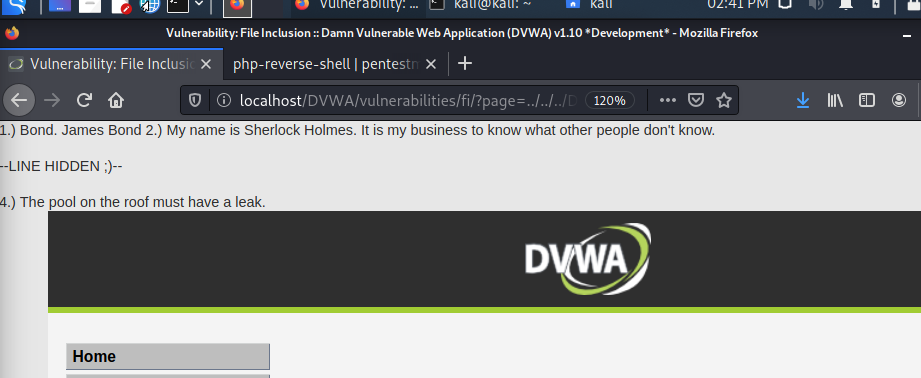
\includegraphics[width=14cm]{img/inclusion/flags.png}
    \caption{Salida de la página escondida}
    \label{fig:hidden}
\end{figure}
Este ataque no funcionará en niveles superiores por qué no permitirán un acceso directo a 
cualquier usuario sin permisos suficientes.
\paragraph{Nivel medio} Probamos a ver si funcionaba el mismo método, pero esta vez fallo.
Por lo que tuvimos que plantear una solución más creativa. Tras reflexionar mucho y no obtener ninguna
solución consideramos que lo más adecuado sería utilizar el {\it reverse shell} creado 
en la sección \ref{sec:upload}. Desde él exploraremos los archivos hasta encontrar la ruta absoluta 
al archivo deseado. El resultado obtenido de esta exploración se ve en la figura \ref{fig:path}.
\begin{figure}[ht!]
    \centering
    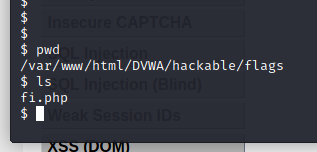
\includegraphics[width=14cm]{img/inclusion/ruta.png}
    \caption{Ruta del archivo buscado.}
    \label{fig:path}
\end{figure}
Probamos con la siguiente entrada para ver si funciona con la ruta absoluta.
\begin{lstlisting}
http://localhost/DVWA/vulnerabilities/fi/?page=/var/www/html/DVWA/hackable/flags/fi.php
\end{lstlisting}
El resultado fue satisfactorio obteniendo el resultado de la figura \ref{fig:hidden}, debido a que la contramedida implementada posiblemente
fuera no permitir rutas relativas mediante una expresión regular. 
No funcionará este método en niveles más altos si nos verifican mediante una expresión
regular la ruta absoluta correcta.
\paragraph{Nivel alto} En este nivel probamos con la misma dirección que en el nivel medio, pero no funcionó.
Esta no supimos sacarla sin mirar el codigo fuente, en el cual comprobaba que el archivo empieza con la secuencia 
de caracteres "file", ya que los tres archivos ofrecidos cumplen esa cualidad. La solución encontrada fue 
usar poner el protocolo file delante del nombre de tal forma que el parámetro {\it page} de la {\it query} 
adquiere el valor:
\begin{lstlisting}
file:///var/www/html/DVWA/hackable/flags/fi.php
\end{lstlisting}
Tras esta petición se obtiene  de nuevo la figura \ref{fig:hidden} como resultado.